\documentclass[14 pt]{extreport}

\usepackage{extsizes}
\usepackage[utf8]{inputenc} %pour accents
\usepackage[T1]{fontenc}	%pour accents
\usepackage[francais]{babel}%pour langue
%\usepackage[textwidth=18cm,textheight=22cm]{geometry} %mise en page
\usepackage{hyperref}	%URL
\usepackage{listings}	%code
\usepackage{amsmath}
\usepackage{graphicx}
\usepackage{epstopdf}
\usepackage{lipsum}
\usepackage{smile_template}
\usepackage{fancyvrb}
\usepackage[section]{placeins}
\usepackage{float}% If comment this, figure moves to Page 2
\epstopdfsetup{outdir=./}

\usepackage{fancyhdr}


\pagestyle{fancy}
\setlength{\unitlength}{1mm}
\addtolength{\headheight}{1.5\baselineskip}
\renewcommand{\headrulewidth}{0.4pt}
\renewcommand{\footrulewidth}{0.4pt}
\rhead{
%
\includegraphics[width=3cm]{images/Logo_Smile_400.jpg}
}

% Redefine the plain page style
\fancypagestyle{plain}{%
  \fancyhf{}%
  \fancyfoot[C]{\thepage}%
  \renewcommand{\headrulewidth}{0pt}% Line at the header invisible
  \renewcommand{\footrulewidth}{0.4pt}% Line at the footer visible
}

\title{\textbf{Rapport de stage de fin d'études}}
\author{Martin Guilloux}


\begin{document}

\maketitle

\section*{Résumé}
Dans le cadre de ma dernière année d'études à l'INSA Centre-Val-de-Loire, j'ai effectué un stage de six mois, l'aboutissement de trois ans passés à l'institut. J'ai effectué ce stage au sein de l'équipe Outsourcing de l'entreprise Smile, à Montpellier. Smile est une entreprise d'hébergement et de développement de websites/webservices française, s'appuyant pour cela sur le monde de l'Open Source.

Ce stage m'a fait expérimenter plusieurs technologies, notamment liées à l'automatisation et à la virtualisation.

\section*{Remerciements}
Je remercie mon enseignant référent Benjamin NGUYEN, d'avoir encadré le déroulement de mon stage.\\
Merci également à Mathieu BLANC, mon maître de stage, pour sa bonne humeur et ses bons conseils.\\
Je remercie aussi toute l'équipe Outsourcing de Smile Montpellier, pour l'accueil et la bonne ambiance quotidienne : Syben, Daber, Adbig, Cebri, Wibru, Secal, Jocor, Dyfei, Segir, Mohla, Aulem, Flmag, Pamar, Alniz, Niper, Alwie, merci d'avoir été plus que de simple collègues de travail.\\
Merci aussi à tout le reste de l'équipe Smile Outsourcing, avec qui j'ai discuté au quotidien.


\tableofcontents

\chapter*{Summary, keywords}
\section*{Summary}
\lipsum[1]\lipsum[1]
\section*{Keywords}
\lipsum[1]


\chapter*{Glossaire}

\begin{itemize}

\item{\textbf{Automatisation}}: Ensemble de techniques permettant le déroulement autonome d'un système, en interconnectant plusieurs élements de ce système ; Par exemple, la génération d'un fichier pdf et l'envoi de ce fichier par mail, tout ceci sans intervention directe humaine.

\item{\textbf{Container}}: système d'exploitation isolé à l'intérieur d'un autre système, permettant ainsi à un hôte de virtualisation de faire tourner plusieurs systèmes sur une seule machine physique. (ex. de systèmes de conteneurisation : docker, lxc, openVZ)

\item{\textbf{Orchestration}}: Processus automatique d'organisation, de coordination et de gestion de systèmes informatiques, de middlewares et de services.

\item{\textbf{Ansible}}: Plate-forme logicielle d'automatisation Open Source en python, détenue par Red Hat. Ansible s'appuie sur ssh et utilise un modèle agentless ne nécessitant pas d'installer un client sur chaque noeud géré.

\item{\textbf{Puppet}}: Une autre plate-forme logicielle d'automatisation Open Source, écrite en ruby, développée par Puppetlabs. Puppet est basé sur un modèle master-slaves, il est nécessaire d'installer un agent sur chaque noeud, qui exécute le catalogue d'instruction envoyé par le puppetmaster.

\item{\textbf{PXE}} (prononcé Pixie): Système permettant à un serveur de booter sur une image de système d'exploitation présente sur le réseau

\item{\textbf{ENC}}: Pour External Node Classifier - Programme externe à Puppet interrogé par le puppetmaster, chargé de gérer pour chaque noeud la liste des classes et des paramètres qui lui sont attribués. (Par exemple, l'outil puppet-dashboard, en plus de fournir une interface web de résumé des puppet run, offre aussi la possibilité d'être utilisé comme ENC)

\end{itemize}

\chapter{Introduction}

\section{Cadre et objectifs du stage}

\subsection{Le stage}L'intitulé de mon stage, "Industrialisation des méthodes de déploiement de plates-formes d'hébergement Internet", suggère la mise en place et la convergence de plusieurs outils pour améliorer à la fois les temps de traitement et la qualité des déploiements de plates-formes d'hébergement. Dans cette optique le travail a été décomposé en plusieurs phases, la première consistant à comprendre le fonctionnement du système existant, l'architecture réseau des serveurs de production de Smile, la base technique en place, ainsi que le périmètre impacté par l'ensemble des modifications à apporter. Il a fallu ensuite mettre en place ou améliorer des solutions dans un souci d'amélioration continue, tout en maintenant et en adaptant l'existant de manière à permettre la cohabitation entre les systèmes de production d'aujourd'hui et de demain.

Avant de parler plus en détail des tâches que j'ai été amené à accomplir, une présentation de l'entreprise qui m'a accueilli pendant ces six mois.

\subsection{Présentation de Smile}
\lipsum
Historique

Description offre commerciale

\chapter{Découverte du réseau de production et de la base technique}

A mon arrivée chez Smile, j'ai commencé par effectuer un tour des technologies utilisées, ainsi que du réseau de production sur lequel j'allais être appelé à travailler. J'ai ainsi pu dégager les points sur lesquels il faudrait agir et isoler les problématiques des différents composants du système de production.

En parallèle je me suis documenté sur les technologies et les outils que j'allais utiliser tout au long de mon stage, notamment Puppet et Ansible.

\section{Présentation du réseau de production}

Les serveurs de production de Smile sont répartis sur trois \emph{datacenters} : Deux dans les environs de Paris (Equinix PA3 à Saint-Denis et Iliad à Vitry-sur-Seine), et un à Lyon (Datacenter SFR à Venissieux) rajouté récemment suite au rachat par Smile de OpenWide Outsourcing (OWO). La convergence avec OWO étant en cours, j'ai été amené à travailler uniquement sur des serveurs présent dans les DC de Paris. Dans chacun de ces deux DC se trouve un Core Router Cisco (cr1 et cr2) ainsi que deux firewalls (fw3,4 et fw5,6), à savoir des serveurs dell sous openBSD. Cette répartition entre plusieurs DC fait suite à la volonté de Smile de mettre en place un Plan de Reprise d'Activité (PRA) incluant des \emph{datacenters} distants de plus de trente kilomètres.

Les core routers et les firewalls sont interconnectés entre les deux sites par fibre optique et administrés sur un vlan spécifique, de même que les serveurs derrière les firewalls (sur un autre vlan).

\begin{figure}[htp]
\centering
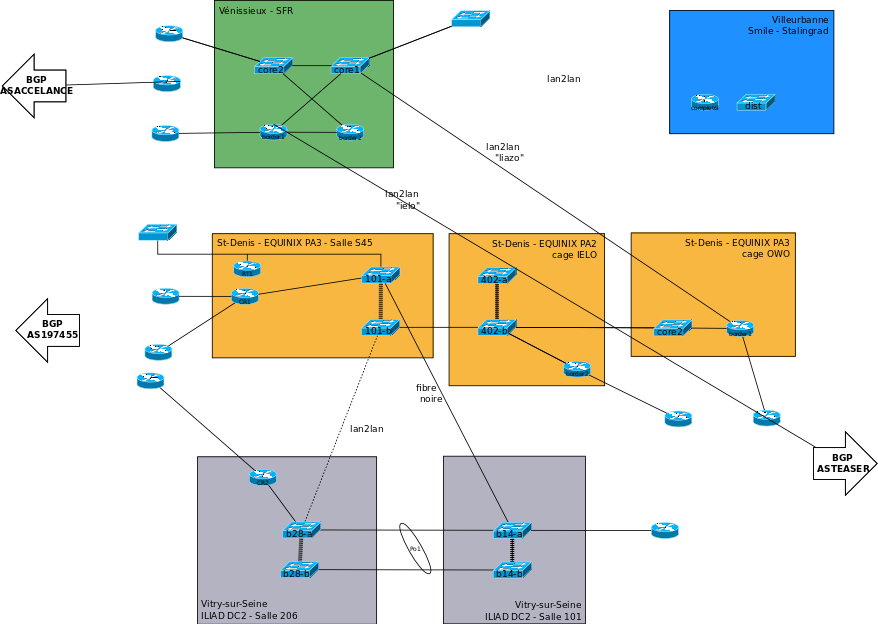
\includegraphics[scale=0.4]{reseau_backbone.png}
\caption{Schéma récapitulatif du réseau backbone de Smile}
\label{}
\end{figure}
%TODO insérer schéma réseau Smile
\section{Le socle technique de la production}

Je vais ici présenter un résumé des technologies utilisées par le système de production chez Smile, en deux parties : les technologies de virtualisation et le système de monitoring, et enfin le système d'orchestration en place, utilisant puppet dont je présenterai rapidement le fonctionnement.
\subsection{Technologies de virtualisation et de monitoring}
\paragraph{Virtualisation :}Les sites hébergés par Smile le sont dans des containers openVZ, avec pour hôtes de virtualisation des serveurs physiques tournant sous CentOS. Les VM sont nommées en fonction du client et du rôle qu'elles jouent dans le système du site web (par exemple youboost-postgresdb1.priv.smile-hosting.fr pour une VM de base de donnée de youboost, ou gifi-pp.priv.smile-hosting.fr pour une VM de pré-production). Les hôtes de virtualisation quand à eux sont nommés en fonction du client dans le cas d'un serveur dédié (ex. gifi-host3.vpn.ti.smile.fr) ou shared-host dans le cas de serveur mutualisé (les serveurs mutualisés sont cependant appelés à migrer vers un cluster utilisant KVM).

Le déploiement de nouveaux hôtes de virtualisation se faisait en PXE, puis sa configuration se faisait à la main ou par le biais de scripts shell.

%TODO schéma openVZ

\paragraph{Monitoring :}Le système de production possède plusieurs facettes qui nécessitent d'être monitorées : Il faut surveiller le bon fonctionnement des backups (basés sur bacula et des scripts utilisant rsync), mais aussi la charge réseau entre les différents datacenters (et potentiellement répartir la charge entre les deux DC), et enfin l'état de tous les serveurs de production.

Pour cela plusieurs outils sont utilisés : Pour les backups un outil interne remonte les informations sur l'état des backups via une page web, tandis que la charge réseau est surveillée via snmp et graphée avec \emph{Cacti}. Pour monitorer l'état des serveurs, enfin, Smile utilise un fork de \emph{Nagios} écrit en python : \emph{Shinken} ainsi qu'une interface web pour afficher ses données, \emph{Thruk}. L'équipe de production utilise également un outil interne de monitoring, \emph{suri5} pour monitorer les sites clients et pour remonter des alertes. Tous ces logiciels sont bien sûr Open Source (un mouvement fortement ancré dans le fonctionnement de Smile, même si cette tendance semble évoluer ces derniers temps).

\subsection{Présentation du système d'orchestration}

Le système d'orchestration à mon arrivée était entièrement basé sur Puppet, un système d'automatisation et d'orchestration Open Source édité par Puppetlabs et écrit en Ruby que je vais rapidement présenter.

Puppet est basé sur un système \textbf{agent-serveur}, c'est à dire que sur chaque noeud géré par puppet il faut installer un \textbf{agent} puppet (présent dans le paquet puppet de base) et le configurer pour se connecter au puppetmaster, le serveur gérant chaque noeud. Un service lance l'agent toutes les heures en temps normal, mais sur une architecture telle que celle de Smile, les temps de traitement excèdent cette durée, c'est donc un \emph{cron} qui lance une \emph{puppet run} deux fois par jour pour éviter la surcharge du puppetmaster (cette cron est générée elle-même lors de chaque run puppet, comme je l'expliquerai un peu plus loin)

Lors de cette run, l'agent se connecte au puppetmaster de manière sécurisée (la suite puppet inclut une autorité de certification qui permet d'ouvrir des connexions sécurisées par SSL). Une fois cette étape d'authentification effectuée, l'agent rassemble des informations sur le système sur lequel il s'exécute. Il envoie ensuite ces informations au puppetmaster, qui s'en sert pour génerer une série d'instructions qui sont renvoyées à l'agent, ce dernier les exécutant et renvoyant en fin de run un résumé de l'état de sortie de chaque instructions, permettant de constater les erreurs de traitement ou les fichiers modifiés (par exemple).

Ci-après, un schéma récapitulatif des interractions au cours d'une puppetrun. On peut constater que la run a lieu en trois temps, d'abord une connexion agent $\rightarrow$ master, pendant laquelle le noeud envoie ses informations (des \emph{facts}), puis master $\rightarrow$ agent, durant laquelle le puppetmaster envoie le catalog au noeud, et enfin une dernière connexion agent $\rightarrow$ master pour le reporting.

\begin{figure}[H]
\centering
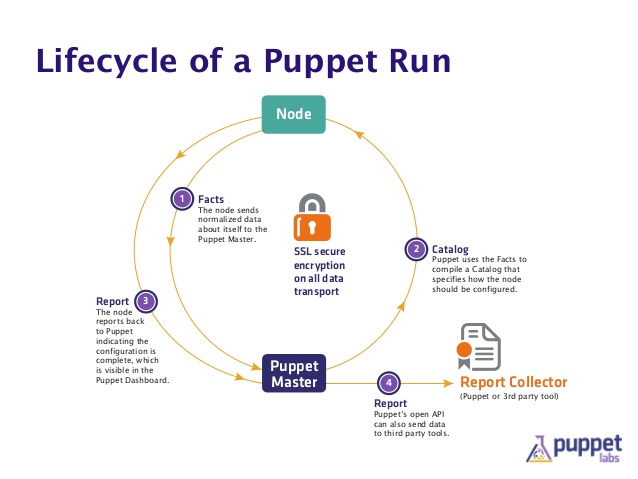
\includegraphics[scale=0.70]{puppetrun.jpg}
\caption{schéma volé éhontément dans une keynote puppetlabs}
\label{}
\end{figure}

Avant de poursuivre, il est nécessaire d'introduire un peu de vocabulaire spécifique à puppet.

Pour savoir quelles instructions exécuter sur un noeud, puppet utilise un système de \emph{manifests} écrits en "langage puppet", un langage à la syntaxe assez spécifique (voir un exemple de manifest puppet en annexe 1) mais relativement simple à comprendre, ainsi qu'un système de \emph{templating} basé sur \emph{erb} (Embedded RuBy) pour pousser des fichiers de configuration sur les noeuds. Ces manifests se divisent en classes, elles-mêmes divisées en ressources. Avec puppet, tout est ressource.\footnote{Paracelse ajouterait que "rien n'est ressource, c'est la dose qui fait la ressource."} Une ressource est en effet l'unité fondamentale d'instruction en puppet. Par exemple, déclarer une ressource de type \emph{file} dans un manifest donnera l'instruction de transférer un fichier (depuis le puppetmaster ou n'importe quelle URI, ou encore d'après un template), tandis qu'une ressource \emph{exec} permettra d'exécuter une commande directement dans le shell de la machine distante (encore une fois, voir en annexe 1 pour un exemple de code puppet)

\begin{itemize}
	\item Une classe est une suite de déclarations de ressources, qui peut être incluse dans un manifest (et ainsi éviter de retaper le même code plusieurs fois) avec des paramètres spécifiés lors de l'écriture de la classe. Par exemple une classe xmpp::client pourrait recevoir un paramètre pour savoir à quel serveur xmpp le client doit se connecter, afin de gérer les fichiers de configuration xmpp correctement.
	\item Un manifest, quant à lui, est un ensemble de ressources et d'inclusions de classes, en somme un fichier puppet générique.
	\item Un module Puppet est un ensemble de manifests, de fichiers, de répertoires et de templates rassemblés dans un but de portabilité. Il peut aussi contenir des fichiers ruby exécutés sur l'hôte distant pour générer des \emph{facts} supplémentaires.
	\item Un catalog Puppet est un ensemble d'instructions envoyées par le puppetmaster à un noeud après les avoir "compilées".
\end{itemize}

Ci-dessous, l'arborescence typique d'un module puppet.
\newpage
\begin{Verbatim}[fontsize=\tiny]
magui@puppetmaster-v4:~/puppet/modules/puppetnode (bacula-lxc)$ tree
.
+-- files
|   +-- etc
|   |   +-- profile-lenny.default
|   |   \-- profile-lenny.puppet
|   +-- etc-default-puppet
|   +-- nrpe
|   |   \-- check_puppet.sh
|   +-- puppet.conf.preprod
|   +-- puppet.conf.prod
|   +-- puppet-cron-cleaning-tasks
|   +-- puppetlabs-pinning
|   \-- tools
|       \-- facter
|           \-- util-ip-patched.rb
+-- lib
|   \-- facter
|       +-- all_vzchildren_fqdn.rb
|       +-- interfaces_with_link.rb
|       +-- lamp_stack_versions.rb
|       +-- majdistrelease.rb
|       +-- pam_bash_users.rb
|       +-- puppetrun_cronjob.rb
|       +-- resolv_domain.rb
|       \-- utc_offset_hours.rb
+-- manifests
|   +-- announce
|   |   \-- register.pp
|   +-- announce.pp
|   +-- collector.pp
|   +-- config.pp
|   +-- cron.pp
|   +-- init.pp
|   +-- nrpe.pp
|   +-- puppetscript.pp
|   +-- service.pp
|   \-- tools
|       +-- all.pp
|       +-- facter.pp
|       +-- lsbrelease.pp
|       +-- puppetlabs_repository.pp
|       \-- ruby.pp
+-- metadata.json
\-- templates
    +-- collector-cron.part.erb
    +-- cron-smile-puppet.erb
    \-- puppet.conf.erb

\end{Verbatim}

\newpage
Une autre composante essentielle du système d'orchestration de Smile est l'utilisation de \emph{hiera}. Il s'agit d'un système permettant de stocker des variables en dehors des manifests dans des fichiers yaml. Dans le cas de Smile hiera est utilisé pour stocker les variables spécifiques à chaque serveur, permettant de gérer les spécificités de chaque machine de manière centralisée.

Lors d'une run puppet, le puppet-dashboard de Smile fait office d'ENC\footnote{voir le glossaire} pour déterminer quelles classes appliquer à chaque noeud. Il lit ensuite les manifests et les hieradata et les adapte au noeud en renseignant les variables (on pourrait faire une analogie avec l'étape des directives de préprocesseur dans une compilation), avant d'envoyer un \emph{catalog} au noeud qui les exécute.

Au cours de cette exécution puppet remplit des fichiers de configuration, installe des paquets à des versions spécifiques, transfère des fichiers de scripts, lance des services... A la fin d'une run puppet, on a donc un système dans un état donné, et refaire une run sans modifier de paramètre garde le serveur dans cet état (ou l'y remet si des fichiers ont été modifiés à la main). Cette idempotence est l'un des points majeurs sur lesquels puppet insiste : Il garantit une infrastructure dans un état stable, exempte de modifications à la main, et apporte donc des certitudes quant à l'état des configurations de chaque système.

\chapter{Les évolutions apportées}

Lors de mon arrivée chez Smile, l'équipe Infra, que j'ai intégré, était en pleine restructuration du fonctionnement interne. Nous avons ainsi mené plusieurs projets en parallèle que je vais présenter ici, notamment la mise en place d'un serveur puppetmaster en version 4 et la migration des modules puppet utilisés par smile, jusque là en version 2 ou 3 ; L'intégration de l'outil d'automatisation \emph{Ansible} au système d'orchestration de la production ; Et une étude pour déterminer le nouveau socle de virtualisation de Smile.

\section{Choix du socle de virtualisation}

Jusqu'ici, le socle de virtualisation utilisé par Smile était, comme décrit plus haut, une base CentOS comme système d'exploitation, et la suite OpenVZ pour déployer des containers. Cependant, le projet OpenVZ apporte son lot de contraintes : il nécessite un kernel spécial (vzkernel) sur l'hôte de virtualisation, et son développement s'est considérablement ralenti ces dernières années. Il a donc fallu réfléchir à la mise en place d'un autre socle de virtualisation avec plus de dynamique dans son développement, et idéalement plus d'avantages que son prédécesseur.

L'utilisation de containers plutôt que de machines virtuelles type KVM/QEMU s'est imposée pour des raisons de performances : L'écart de performances entre un container et un OS "bare-metal" est de l'ordre de 2 à 3\%, contre 5-6\% environ pour une machine type KVM. En termes de densité, il est possible de peupler un serveur avec 14 fois plus de containers que de KVM.

Notre choix s'est porté sur l'utilisation de LinuX Containers (\emph{lxc}), avec son \emph{daemon} lxd. Ce système de conteneurisation a depuis quelques années le vent en poupe, bénéficiant d'une intégration privilégiée au noyau Linux, dont il tire profit avec des features comme les cgroups et les espaces de nommages, qui permettent d'apporter une couche supplémentaire de sécurité aux containers. 

Cependant lxd, étant un produit de Canonical, n'est disponible que sous Ubuntu. C'est pourquoi il a été arrêté que les nouveaux hôtes de virtualisation de Smile sont maintenant sous Ubuntu Server 16.04, l'édition Long Term Support de Ubuntu Server.

\section{Intégration d'Ansible}

Un autre projet dans le cadre de l'amélioration et l'industrialisation de la production, nous avons intégré l'utilisation d'Ansible à l'ensemble des outils de Smile, que je vais brièvement présenter ici.
\newpage
\subsection{Présentation d'Ansible}

\subsubsection{Présentation générale}
Ansible est un "outil d'automatisation simple"\footnote{Du moins d'après ses concepteurs : \url{https://www.ansible.com/}}, fonctionnant sans agent au contraire de Puppet. Pour les noeuds à administrer, il suffit d'avoir un daemon ssh ainsi que l'interpréteur python installé. 

Ansible utilise ensuite une série de connexions ssh pour pousser des scripts python qui s'exécuteront sur le noeud. On a donc une architecture beaucoup plus simple que celle de Puppet puisqu'il suffit d'installer Ansible sur son poste pour pouvoir gérer immédiatement toutes les machines de production. En termes de sécurité, Ansible s'appuie sur openSSH, qui fait office de référence en termes de shell distant.

\subsubsection{Fonctionnement}

Ansible utilise un fichier \emph{inventory} dans le style des fichiers ini (exemple ci-après) pour faire le lien entre un nom et un groupe de machines comme suit :
\begin{framed}
\begin{Verbatim}[fontsize=\scriptsize]
[webservers]
foo.example.com
bar.example.com

[dbservers]
one.example.com
two.example.com
three.example.com

[targets]
localhost ansible_connection=local
other1.example.com ansible_connection=ssh ansible_user=mpdehaan
other2.example.com ansible_connection=ssh ansible_user=magui
\end{Verbatim}
\end{framed}
Pour effectuer des actions sur un groupe il suffit de lui préciser par exemple \begin{framed}magui@fonzie:~\$ ansible -m ping targets\end{framed}

L'option -m ping permet d'exécuter un seul module Ansible sur les cibles (ici le groupe \emph{targets}). Le module ping est un simple module qui détermine si une machine est atteignable et si python est installé dessus.

Le fichier d'inventory par défaut est stocké dans /etc/ansible/inventory. Il est également possible d'utiliser un fichier alternatif par exemple avec :

\begin{framed}magui@fonzie:~\$ ansible -i /mnt/nfs/ansible/shared\_inventory -m ping targets\end{framed}

Ansible se voulant plus simple que Puppet ou d'autres outils d'automatisation, les instructions à lui passer n'utilisent pas de système de classe ou d'ENC. L'ensemble des instructions peut être soit passé directement en lignes de commandes (pour exécuter un seul module comme plus haut), soit dans un fichier yaml appelé \emph{playbook}. Un playbook décrit l'ensemble des \emph{modules} et des \emph{rôles} à exécuter, ainsi que les groupes de machines sur lesquels exécuter ces modules et ces \emph{modules}.\footnote{Un exemple de playbook Ansible est disponible à la fin de ce rapport, en annexe 2}

\begin{figure}[htp]
\centering
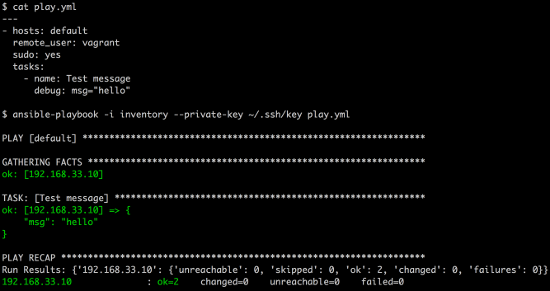
\includegraphics[scale=1.10]{play.png}
\caption{Un exemple d'exécution de playbook Ansible}
\label{}
\end{figure}

Un playbook peut contenir plusieurs \emph{plays}, qui sont un ensemble d'instructions exécutées sur un groupe de machines. Il est donc possible de configurer plusieurs types d'hosts en une seule run Ansible, contrairement à Puppet. Par exemple, au début de mon stage, l'ajout d'un noeud à l'architecture gérée par Puppet nécessitait de se logger sur le noeud, de lancer une première run puppet afin de générer une CSR (Certificate Signing Request) à l'intention de l'autorité de certification du puppetmaster, puis de se connecter sur le puppetmaster pour signer à la main cette CSR, et enfin de se reconnecter au noeud pour faire une run puppet effective. Grâce à un playbook Ansible conçu durant mon stage et contenant trois plays successives (une sur le noeud, une sur le puppetmaster et une deuxième sur le noeud), il est désormais possible d'effectuer toutes ces tâches en une seule commande ansible.

Comme Puppet, l'idempotence est une notion importante avec Ansible, plusieurs runs successives exécutées sur le même serveur devant retourner le même état. On peut donc être certain de l'état d'un système à l'issue d'une run vis-à-vis des configurations et des paquets installés.

\paragraph{}Un \emph{module} Ansible est l'unité d'instruction d'Ansible. Un module est comparable à une ressource Puppet, chaque module correspondant à un script python poussé par Ansible sur les noeuds pendant une run. Il existe de nombreux modules, des plus génériques (un module \emph{raw} pour exécuter une commande ssh directe (peu recommandé)) aux plus spécifiques (par exemple \emph{rabbitmq\_plugin} pour ajouter des plugins au système de messages queue RabbitMQ)

Il est possible de rassembler un ensemble de tasks (suite d'instructions, et donc de modules), de templates, et de fichiers de variables dans une structure en arborescence appelée \emph{rôle Ansible}. On peut comparer un rôle Ansible à un module Puppet, bien que son arborescence soit un peu plus complexe, puisqu'elle ajoute des répertoires de tests, de valeurs par défaut et de handlers.

Les handlers sont des instructions appelées à l'exécution d'une instruction spéciale dans une play, l'instruction \emph{notify}. Par exemple, on peut, dans un playbook, installer un serveur web apache et pousser sa configuration à l'aide d'une template, en ajoutant l'instruction \emph{notify} lors du transfert du fichier de configuration, avec un paramètre (par exemple) "apache-reload". Si le handler du même nom est présent dans le dossier éponyme du rôle, ses instructions sont exécutées dans la foulée (dans notre cas, on reload la configuration apache juste après l'avoir modifiée)

Un rôle Ansible peut de plus être versionné sur un serveur git. Il est alors possible de l'appeler en utilisant un outil appelé ansible-galaxy, qui ira alors chercher automatiquement la dernière version du rôle. Ce système de partage des rôles permet à la fois de bénéficier de mises à jour régulières mais aussi de simplement inclure différents rôles plutôt que de réécrire un playbook à chaque fois. Par exemple, le playbook suivant installe et configure une stack Kibana + Elastic Search + Logstash uniquement en important et en exécutant des rôles Ansible :

\begin{framed}
\begin{Verbatim}[fontsize=\scriptsize]
- hosts: logs
  gather_facts: yes
  
  vars_files:
    - vars/main.yml
  pre_tasks:
    - name: Update apt cache if needed.
	  apt: update_cache=yes cache_valid_time=86400
  roles:
    - geerlingguy.java
	- geerlingguy.nginx
	- geerlingguy.elasticsearch
	- geerlingguy.elasticsearch-curator
	- geerlingguy.kibana
	- geerlingguy.logstash
	- geerlingguy.logstash-forwarder
\end{Verbatim}
\end{framed}

Cependant, au contraire de Puppet, les solutions permettant de centraliser les run et les logs Ansible à la manière d'un ensemble puppetmaster + puppetdashboard sont soit trop peu performantes, soit non Open Source et aux tarifs dissuasifs : C'est le cas notamment de la solution Ansible Tower détenue par RedHat pour centraliser une architecture d'automatisation Ansible : Le prix des licenses est suffisament élevé pour décourager l'utilisation chez Smile, et la libération des sources, si elle semble prévue par RedHat, n'a aucune date annoncée.

\subsubsection{Intégration d'Ansible à la production de Smile}

Dès mon arrivée chez Smile j'ai pu découvrir Ansible en profondeur, notamment à l'aide du très bon Ansible for DevOps\footnote{Jeff Geerling, Leanpub, 2016-11-23}, dans le but d'automatiser les processus de déploiements de plates-formes. L'une de mes premières missions chez Smile a été d'adapter un script chargé de configurer un \emph{bonding} entre deux interfaces ethernet aux dernières versions de CentOS ainsi que la configuration de bridges et de vlans. J'ai finalement migré le comportement de ce script vers Ansible, à la fois pour me permettre de mieux appréhender son fonctionnement mais aussi pour que, couplé à un déploiement d'OS en PXE, il soit possible d'automatiser entièrement le déploiement et la configuration réseau d'un nouveau serveur hôte de virtualisation. Une fois qu'a été actée la décision de passer nos nouveaux hôtes de virtualisation sous Ubuntu, ce rôle Ansible a simplement eu besoin d'être adapté pour inclure les templates de fichiers de configuration réseau de type /etc/network/interfaces.d (utilisées par Ubuntu) en plus des templates destinées aux machines sous CentOS.

J'ai ainsi pu commencer à discerner les avantages et les inconvénients d'Ansible, ainsi que ses limitations. J'ai notamment été un peu déçu par les limitations induites par le yaml, langage utilisé pour écrire les playbooks Ansible. Si plusieurs structures de contrôle sont mises en place - équivalent d'un test \emph{if} avec la ligne \emph{when} ajoutée à la fin de l'appel d'un module, possibilité d'exécuter des blocs de modules, possibilité d'appeler du code python sur les variables du playbook - le langage manque clairement de possibilités du point de vue programmation. Ce point faible fait partie intégrante de la philosophie d'Ansible : "Faire générique", s'adapter au plus grand nombre plutôt qu'aux cas particuliers. Cependant cette limitation apporte des contraintes assez lourdes, compliquant des tâches pourtant assez simples dans un shell comme par exemple effectuer l'équivalent d'un \begin{verbatim}for i in $(ls /home/fonzie); do cat $i>> /tmp/singeDuFutur.out \end{verbatim} 

En effet, pour faire une boucle sur des fichiers ou autres, il faut les lister de la manière suivante :

\begin{framed}
\begin{Verbatim}[fontsize=\scriptsize]

    # emit a debug message containing the content of each file.
    - debug:
        msg: "{{ item }}"
      with_file: # peut apparaître sous la forme "with_items"
        - first_example_file
        - second_example_file
        
\end{Verbatim}
\end{framed}

On peut donc voir que pour certaines tâches, Ansible demande des tweaks et des contorsions pour arriver à ses fins. Cependant il permet dans l'ensemble de déployer des configurations et des outils très rapidement une fois les rôles codés, ce qui a justifié le choix de l'utiliser pour déployer les hôtes de virtualisation de Smile ainsi que la base d'outils. 

\lipsum[1]
\lipsum[1]
\lipsum[1]
\lipsum[1]

\section{Upgrade de puppet}
\lipsum[1]
\lipsum[1]
\lipsum[1]
\lipsum[1]


\chapter{Autres missions}
\lipsum

\chapter{Conclusion, bilan}
\lipsum

\end{document}
